\documentclass[a4paper,10pt]{article}

\usepackage[activeacute]{babel}
\usepackage[utf8]{inputenc}
\usepackage{bookman}
\usepackage{color}
\usepackage{graphicx}
\usepackage{anysize}
\usepackage{multicol}
\usepackage{tgcursor}
\usepackage[pdftex=true,colorlinks=true,linkcolor=black,urlcolor=blue]{hyperref}

\marginsize{1.5cm}{1.5cm}{1.5cm}{1.5cm}
\newcommand{\HRule}{\rule{\linewidth}{0.5mm}}

\date{}

\pagenumbering{arabic}
\setcounter{page}{1}

\begin{document}

% ===================================== MEMBRETE ===================================== %
\begin{center}
  \textsc {
    Universidad Simón Bolívar \\[0cm]
    Departamento de Computaci\'on y Tecnolog\'ia de la Informaci\'on \\[0cm]
    CI5438 - Inteligencia Artificial I \\[0cm]
    Trimestre Abril - Julio 2021 \\[0cm]
    Prof. Carlos Infante \\[0cm]
    Amin Arriaga 16-10072, David Segura 13-11341, Wilfredo Graterol 15-10639
  }
  \HRule \\[0.4cm]
  {\Large \textbf{B\'usqueda Informada: A* vs IDA*}} \\[0.4cm]
  \textsc{
    \today
  }
  \HRule
\end{center}

\section{Introducci\'on}
  Las b\'usquedas informadas son algoritmos muy importantes en el
  \'area de inteligencia artificial, a pesar de que hoy en d\'ia 
  la rama m\'as famosa es la de Machine Learning. Entre estos algoritmos,
  A* e IDA* destacan bastante por su rendimiento en distintos problemas, y 
  ambos comparten la car\'acter\'istica de usar una funci\'on \verb|h| llamada 
  \textit{heur\'istica}, el cual toma un estado cualquiera del problema
  y estima el costo de llegar hasta alg\'un estado objetivo. Estas funciones
  deben cumplir varias propiedades, como admisibilidad y consistencia, para
  que puedan ser \'utiles en la resoluci\'on de problemas. Mientras mejor
  sean estas he\'uristicas, m\'as eficiente ser\'an las funciones que lo usan.
  En particular, existen un tipo de heur\'istica llamado Pattern DataBase (PDB)
  que reducen la complejidad del problema original al proyectarlo sobre un 
  espacio de soluciones m\'as peque\~no y almacenan las soluciones de cada 
  posible estado de este nuevo problema en una base de datos, se repite este 
  proceso con distintas proyecciones y luego en el problema original se utilizan
  estos valores almacenados por estados para calcular una heur\'istica. Si las
  proyecciones cumplen que al sumarse siguen cumpliendo las car\'acter\'isticas
  de admisibilidad y consistencia, se dicen que son PDBs aditivas, en caso 
  contraria, se dice que no son aditivas y en general se toma el m\'aximo valor 
  entre todos ellos. En este informe estudiaremos el rendimiento de A* e IDA* con 
  los distintos tipos de poda de duplicados, utilizando PDBs y sobre los problemas
  de N Puzzle, Torres de Hanoi, Top Spin y el Cubo de Rubik en distintas
  dificultades, as\'i como sus \'arboles de b\'usqueda. Nos concentraremos
  en el tiempo de ejecuci\'on, memoria usada y n\'umero de estados por segundos
  generados para realizar el an\'alisis.

\section{Estructura del Repositorio}
  El repositorio presenta la siguiente estructura de archivos:

  \begin{verbatim}
    proyecto-1-ci5437/
    |__ benchmarks/...
    |__ bin/...
    |__ generators
    |   |__ HanoisTowersGenerator.py
    |   |__ SlidingTileGenerator.py
    |   |__ TopSpinGenerator.py
    |__ informe.pdf -> src/L_informe/informe.pdf
    |__ Makefile
    |__ papers/...
    |__ pdbs/...
    |__ psvn/...
    |__ puzzles/...
    |__ README.md
    |__ resources/...
    |__ search_tree/...
    |__ src
        |__ head.hpp
        |__ heuristics.cpp
        |__ heuristics.hpp
        |__ InformedSearchs.cpp
        |__ InformedSearchs.hpp
        |__ L_informe/...
        |__ main.cpp
        |__ Node.cpp
        |__ Node.hpp
        |__ NodesPriorityQueue.cpp
        |__ NodesPriorityQueue.hpp
        |__ PriorityQueue.hpp
  \end{verbatim}

  donde 

  \begin{itemize}
    \item \verb|benchmarks/| contiene los casos de prueba para los distintos 
    puzzles separados en directorios, as\'i como los archivos necesarios para 
    generar nuevos casos de prueba.
  
    \item \verb|bin/| contiene los archivos binarios que resuelven alg\'un puzzle.
    Los archivos en este directorio tienen el formato \verb|P.out| donde \verb|P|
    es el nombre de alg\'un puzzle. Estos archivos no son agregados al repositorio.

    \item \verb|generators/| contiene los generadores de archivos \verb|.psvn|.
    Los que se encuentran actualmente son:
    \begin{itemize}
      \item \verb|generators/HanoisTowersGenerator.py| tal que al ejecutarse con 
      \verb|P > 2| y \verb|D > 1|, imprime un PSVN el puzzle de las Torres 
      de Hanoi con \verb|P| astas y \verb|D| discos.

      \item \verb|generators/SlidingTileGenerator.py| tal que al ejecutarse con 
      \verb|M > 0| y \verb|N > 0|, imprime un PSVN el puzzle de Sliding 
      Tiles con dimensi\'on \verb|M x N|.

      \item \verb|generators/TopSpinGenerator.py| tal que al ejecutarse con 
      \verb|K > 1| y \verb|N > K|, imprime un PSVN el puzzle Top Spin con 
      \verb|N| tokens y un 'turntable' de longitud \verb|K|.
    \end{itemize}

    \item \verb|pdbs/| contiene los archivos necesarios para generar PDBs para los 
    distintos puzzles a estudiar. Revise el archivo \verb|pdbs/README.md| para m\'as
    informaci\'on.

    \item \verb|psvn/| contiene el c\'odigo fuente para compilar la API de PSVN.
    
    \item \verb|puzzles/| contiene archivos \verb|.psvn|.
    
    \item \verb|search_tree| contiene los archivos necesarios para realizar el estudio
    de los \'arboles de b\'usqueda de cada puzzle.

    \item \verb|src/| contiene el c\'odigo fuente principal para compilar y ejecutar 
    los distintos algoritmos de b\'usqueda informada que estudiaremos en este proyecto.
    Daremos una brvee explicaci\'on de cada archivo:
    \begin{itemize}
      \item \verb|src/Node.*| tiene la implementaci\'on de nodo que hemos usado durante 
      las clases. Tambi\'en almacena la profundidad del camino parcial hasta ese nodo.

      \item \verb|src/PriorityQueue.hpp| tiene la implementaci\'on de una cola de 
      prioridad gen\'erica. Permite definir el tipo de dato que servir\'a para realizar 
      las comparaciones, el tipo de los elementos que almacenar\'a y la funci\'on de 
      comparaci\'on. No se separ\'o en archivos \verb|.cpp| y \verb|.hpp| debido a los 
      problemas de C++ con los templates.

      \item \verb|src/NodesPriorityQueue.*| tiene otra implementaci\'on de una cola de 
      prioridad pero basada en nodos, y que adem\'as de los m\'etodos 
      \verb|empty|, \verb|add| y \verb|pop|, tambi\'en tiene los m\'etodos \verb|find|
      que busca un nodo seg\'un el estado que almacena; y \verb|replace_if_less| que,
      dado un nodo, verifica si la cola tiene otro nodo que representa al mismo estado
      que adem\'as tiene un costo parcial superior al nodo par\'ametro, entonces es 
      sustituido por el nodo par\'ametro. Estas 2 funciones en una cola de prioridad 
      com\'un ser\'ian $O(n)$, lo cual no es deseable en las funciones de b\'usqueda.

      \item \verb|src/InformedSearchs.*| tiene las implementaciones de los algoritmos
      de b\'usqueda que se estudian en el proyecto. En particular, se encuentran los 
      siguientes algoritmos:
      \begin{itemize}
        \item A* sobre grafos.
        \item A* sobre \'arboles.
        \item A* con eliminaci\'on tard\'ia de nodos.
        \item IDA* sobre grafos.
        \item IDA* sobre \'arboles.
        \item IDA* con eliminaci\'on parcial de nodos.
      \end{itemize}

      \item \verb|src/heuristics.*| tiene las implementaciones de las distintas 
      he\'uristicas que se usar\'an, principalmente de PDBs.

      \item \verb|src/main.cpp| y \verb|src/head.hpp| el cual, al compilarse y
      ejecutarse, te permite ingresar un estado inicial, as\'i como escoger un
      algoritmo de b\'usqueda y una heur\'istica de los implementados para resolver
      el puzzle. Consulte el archivo \verb|Makefile| para m\'as informaci\'on.
      
      \item \verb|src/L_informe/| contiene los archivos fuentes de latex necesarios 
      para generar este informe.
    \end{itemize}
    
  \end{itemize}

\section{\'Arboles de B\'usqueda}
    En las \textit{Figura 1 y 2} podemos notar que hay una inmensa diferencia entre la 
    cantidad de nodos expandidos por cada puzzle con y sin poda de duplicados, lo
    cual tambi\'en se refleja en el factor de ramificaci\'on mostrado en la 
    \textit{Tabla 1}, que disminuye considerablemente al aplicar la poda. Esto
    nos comienza a indicar la necesidad de aplicar alguna poda en los algoritmos 
    de b\'usqueda. El ejemplo m\'as claro de esto fue el puzzle de las Torres de 
    Hanoi con 12 Discos, donde, sin poda de duplicados, ya expand\'ia alrededor de 
    $10^7$ nodos a profundidad de 10, mientras que con poda se lograron expandir 
    todos los posibles estados, llegando hasta una profundidad de 81 (lo cual nos 
    muestra que podemos almacenar todo el puzzle en un solo pdb). \\
    
    \begin{figure*}[t!]
      \centering
      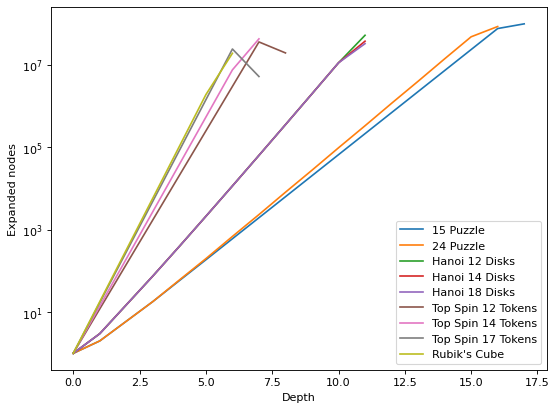
\includegraphics[scale=0.45]{search_tree/search_tree2.png}
      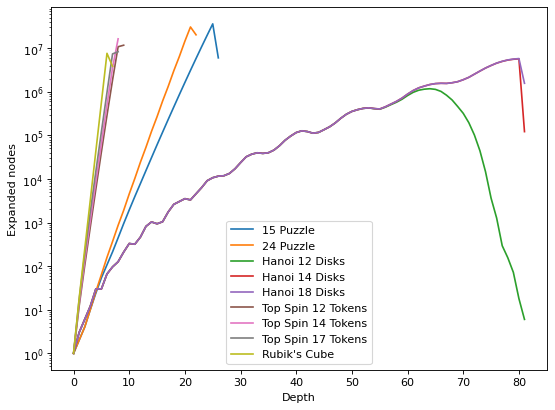
\includegraphics[scale=0.45]{search_tree/search_tree.png}\\
      \textit{\small{Figuras 1 y 2. A la izquierda, los nodos expandidos por profundidad en
      cada puzzle sin poda de duplicados. A la derecha, con poda de duplicados}}\\
      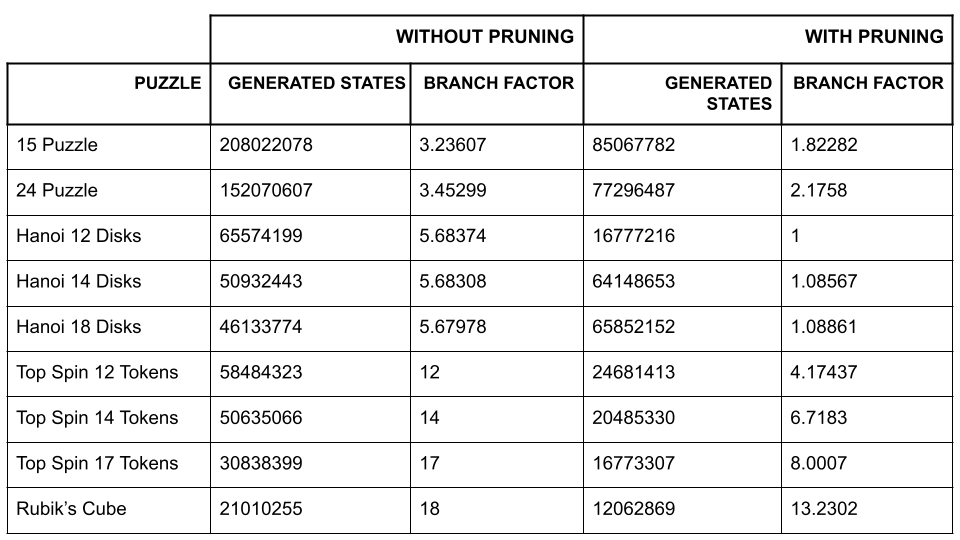
\includegraphics[scale=0.35]{search_tree/table1.png}\\
      \textit{\small{Tabla 1. N\'umero de estados generados y factor de ramificaci\'on
      promedio de cada puzzle con y sin poda de duplicados.}}
    \end{figure*}
    
    Tambi\'en se resalta la diferencia en la cantidad de nodos generados por
    profundidad entre cada puzzle. Tanto los Top Spins como el Cubo de Rubik tienen 
    un crecimiento muy acelerado, alcanzando $10^7$ estados nada m\'as a profundidad
    de 10 con poda de duplicados, mientras que las Torres de Hanoi son los que 
    presentan el crecimiento m\'as lento. Esto no es necesariamente un indicador 
    de dificultad del puzzle, pues alguno podr\'ia crecer lento y llegar a una 
    gran profundidad, mientras que otro crezca r\'apido pero llegar hasta una 
    profundidad baja. Esta medida de crecimiento tal vez es importante 
    en el rendimiento de los distintos algoritmos de b\'usquedas.\\
    
    Otro fen\'omeno interesante que podemos notar en las gr\'aficas es que, para las 
    Torres de Hanoi, los nodos expandidos hasta una profundidad de 60 son iguales 
    para 12, 14 y 18 discos, lo cual es l\'ogico, pues partiendo del estado final
    es imposible mover las piezas m\'as grandes, as\'i que los primeros movimientos
    son exactamente iguales. Eventualmente hasta cierta profundidad las Torres de 
    Hanoi con 14 y 18 discos tamb\'ien ser\'ian exactamente iguales y luego el de 
    14 comenzar\'ia a disminuir la cantidad de nodos expandidos.\\
    
    Por \'ultimo, la cantidad de estados generados por segundo tambi\'en
    cambia dr\'asticamente entre cada puzzle. Se generan alrededor de 7 veces m\'as 
    estados de 15 Puzzle que del cubo de Rubik. Esto se puede deber a varios factores,
    desde longitud en la representaci\'on de los estados de cada puzzle, as\'i como
    la complejidad en las reglas de transici\'on, donde, por ejemplo, las del cubo 
    de Rubik son m\'as dif\'icles de aplicar que la de los N Puzzle. Sin embargo, 
    no tenemos suficiente evidencia para determinar que factores afectan la cantidad
    de estados generados por segundo.
    
    
\section{Casos de Prueba}
  Para cada puzzle se correr\'an los distintos algoritmos sobre 5 casos de pruebas
  con una dificultad lo suficientemente baja como para que no tarden m\'as de 2 
  minutos y se tomar\'a el rendimiento promedio de los algoritmos en cada 
  uno de esos casos. Luego se correr\'a un caso de prueba lo m\'as dif\'icil posible,
  y se graficar\'an los nodos expandidos por cada profundidad. Decidimos usar esta 
  metodolog\'ia para no durar una gran cantidad de tiempo en pruebas d\'ificiles
  y a\'un as\'i obtener datos de distintos casos para evitar que, por mala suerte, 
  usemos uno anormal, d\'andonos datos que no son comunes y lo tomemos como tal.\\
  
  \subsection{15 Puzzle}
    Para el 15 Puzzle usamos como heur\'istica la distancia Manhattan. Los
    5 casos de pruebas f\'aciles y el dif\'icil escogidos junto a la longitud de sus 
    soluciones fueron:
    
    \begin{verbatim}
      3 14 9 11 5 4 8 2 13 12 6 7 10 1 15 B    (46)
      14 1 9 6 4 8 12 5 7 2 3 B 10 11 13 15    (45)
      7 11 8 3 14 B 6 15 1 4 13 9 5 12 2 10    (46)
      12 15 2 6 1 14 4 8 5 3 7 B 10 13 9 11    (47)
      12 8 15 13 1 B 5 4 6 3 2 11 9 7 14 10    (50)
      5 9 13 14 6 3 7 12 10 8 4 B 15 2 11 1    (57)
    \end{verbatim}
    
    \begin{figure*}[t!]
      \centering
      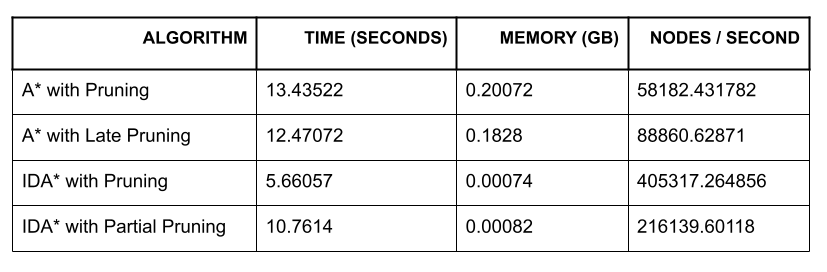
\includegraphics[scale=0.3]{15puzzle/tabla2.png} 
      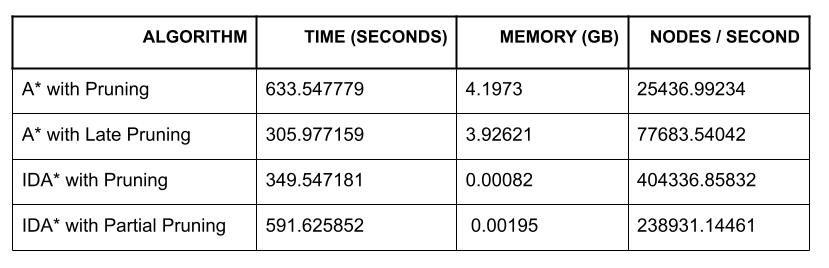
\includegraphics[scale=0.3]{15puzzle/tabla3.png} \\
      \textit{\small{Tablas 2 y 3. A la izquierda promedio de tiempo, memoria y n\'umero 
      de nodos expandidos en los 5 casos de pruebas f\'aciles del 15 Puzzle por cada algoritmo 
      de b\'usqueda. A la derecha tiempo, memoria y n\'umero de nodos expandidos en el caso
      de prueba dif\'icil del 15 Puzzle para cada algoritmo de b\'usqueda.}}\\
      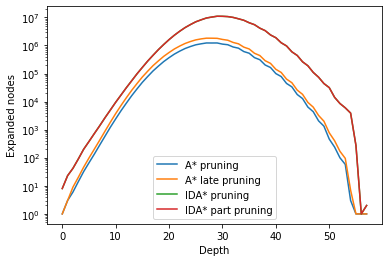
\includegraphics[scale=0.4]{15puzzle/15puzzle_hard.png} \\
      \textit{\small{Figura 3. N\'umero de nodos expandidos por profundidad en el caso 
      de prueba dif\'icil del 15 puzzle por cada algoritmo de b\'usqueda.}}
    \end{figure*}
    
    Podemos notar en las \textit{Tablas 2 y 3} que para los casos f\'aciles IDA* fue mucho 
    m\'as eficiente que A*, siendo el mejor IDA* con poda de duplicados, y el peor A*
    con poda de duplicados. Sin embargo, para el caso dif\'icil, A* con 
    poda tard\'ia de duplicados se vuelve el dominante, probablemente debido 
    al aumento en la profundidad, lo cual se vuelve inconveniente para IDA*. Sin embargo,
    el uso de la memoria para A* fue considerablemente grande, alrededor de 4 GB, mientras
    que el de IDA* es casi despreciable como era de esperar. Tambi\'en podemos confirmar 
    gracias a la \textit{Figura 3} que el n\'umero de nodos expandidos por IDA* es mucho
    mayor que el de A* (note que la gr\'afica est\'a en escala logar\'itmica), pero que 
    el n\'umero de nodos expandidos por segundos es menor en A*. \\
    
    Algo interesante que se ve en la gr\'afica es que el numero de nodos expandidos por 
    IDA* fue exactamente el mismo con poda y poda parcial de duplicados.
    Suponemos que es porque para llegar a un estado repetido puede ser usando el movimiento
    opuesto al \'ultimo movimiento o a trav\'es de una gran cantidad de pasos que generen un
    ciclo, pues no es tan simple como moverse en un c\'irculo. Para el primer caso, la 
    poda parcial es suficiente para evitarlo. Mientras que para el segundo, lo mas 
    probable es que el mismo algoritmo no permita realizar tal circuito, pues requerir\'ia una 
    gran cantidad de movimientos que no ayudan a llegar a una soluci\'on, y por lo tanto 
    alcanzar\'ia un costo que impedir\'ia seguir expandiendo esa rama. As\'i, al s\'olo
    ser necesario podar los estados padres y como A* con poda tard\'ia 
    de duplicados genera m\'as nodos por segundo que con poda de duplicados, 
    se obtiene que A* con poda tard\'ia es mucho m\'as eficiente que la poda total.
    
  \subsection{24 Puzzle}
    Para el 24 Puzzle usamos como heur\'istica PDBs aditivos, particionando
    el puzzle tal como se muestra en la \textit{Figura 4}. Lo 5 casos de pruebas f\'aciles 
    y el dif\'icil escogidos junto a la longitud de sus soluciones fueron:
  
  \begin{verbatim}
      5 1 B 2 4 6 7 8 3 9 10 16 12 13 14 15 22 11 18 19 20 17 21 23 24 (16)
      1 6 7 2 3 5 12 8 B 4 10 17 11 13 9 15 16 18 23 14 20 21 22 24 19 (20)
      5 1 2 3 4 6 7 12 8 9 15 10 11 13 14 21 20 18 B 24 16 22 17 19 23 (20)
      1 2 3 4 9 11 5 10 8 14 6 7 B 12 13 15 16 17 18 19 20 21 22 23 24 (20)
      5 2 7 3 4 10 6 1 8 9 15 11 12 13 14 16 22 21 19 24 20 17 23 18 B (20)
      11 5 7 2 4 B 1 3 8 9 6 10 18 16 14 12 20 13 23 19 17 21 15 24 22 (53)
    \end{verbatim}
    
    Utilizamos estos casos de prueba con poca dificultad pues, a pesar de que las
    m\'aquinas virtuales de \textit{Google Colab} ofrecen una gran cantidad de memoria
    RAM, su procesador es muy lento, por lo que crear casos de prueba que tuvieran
    tiempos de ejecuci\'on m\'as aceptable, como 2 a 5 minutos para los casos f\'aciles,
    es dif\'icil, pues al no saber de antemano la longitud de la soluci\'on, tenemos
    que probar hasta que alcance una o decidamos detener la ejecuci\'on. \\ 
    
    Notamos en las \textit{Tablas 4 y 5} que, al igual que con el 15 Puzzle, IDA* con
    poda de duplicados es la m\'as eficiente para los casos de prueba f\'aciles, pero 
    IDA* con eliminaci\'on parcial de duplicados fue el que tard\'o m\'as. Adem\'as,
    A* con poda total tuvo el mejor rendimiento para el caso dif\'icil, diferiendo de
    15 Puzzle en el que fue A* con poda tard\'ia. A\'un as\'i, se mantiene el patr\'on 
    de que IDA* empeora su rendimiento para los casos dif\'iciles, probablemente por 
    el aumento en la profundidad de la b\'usqueda. \\
    
    La \textit{Figura 5} es muy parecida a la del 15 Puzzle, incluso presenta tambi\'en
    un pico al final para IDA*, mientras que A* termina con una zona plana, indicando
    que para este punto solo expando los nodos necesarios para alcanzar la soluci\'on.
    
  
    \begin{figure*}[t!]
      \centering
      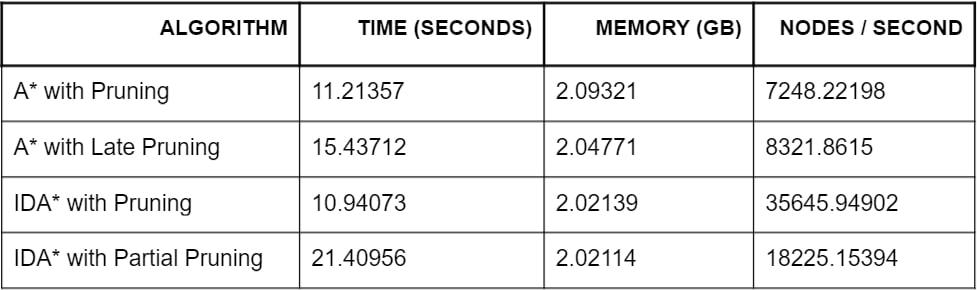
\includegraphics[scale=0.32]{24puzzle/24p_tabla_prom.jpg} 
      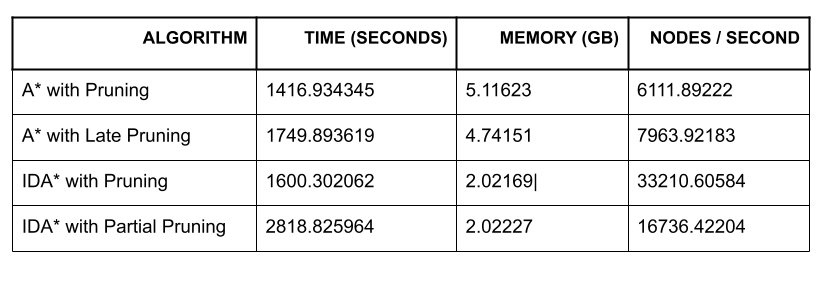
\includegraphics[scale=0.3]{24puzzle/tabla1.png} \\
      \textit{\small{Tablas 4 y 5. A la izquierda promedio de tiempo, memoria y n\'umero 
      de nodos expandidos en los 5 casos de pruebas f\'aciles del 24 Puzzle por cada algoritmo 
      de b\'usqueda. A la derecha tiempo, memoria y n\'umero de nodos expandidos en el caso
      de prueba dif\'icil del 24 Puzzle para cada algoritmo de b\'usqueda.}}\\
      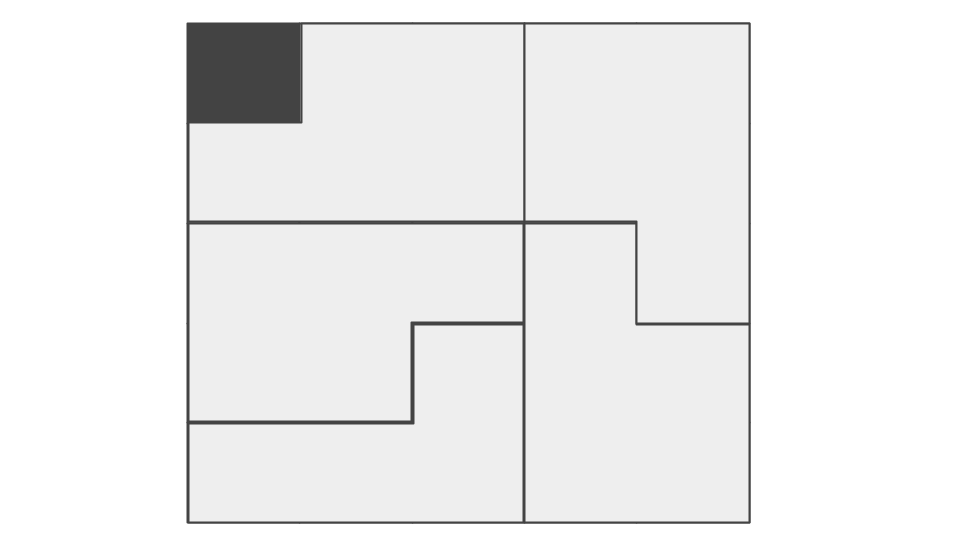
\includegraphics[scale=0.2]{24puzzle/pdb.png}
      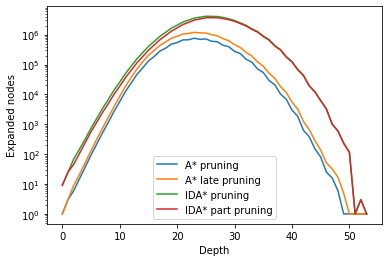
\includegraphics[scale=0.4]{24puzzle/24puzzle_hard.png}
      \\
      \small{\textit{Figuras 4 y 5. A la izquierda, partici\'on del 24 Puzzle
      que usamos para generar los Pattern Data Bases. A la derecha, N\'umero 
      de nodos expandidos por profundidad en el caso de prueba dif\'icil del 
      24 puzzle por cada algoritmo de b\'usqueda.}}
    \end{figure*}

  \subsection{Towers of Hanoi 4 Pegs - 12 Disks}
    Tal como mencionamos en la secci\'on 3, pudimos confirmar que todo el puzzle de las
    Torres de Hanoi con 12 Discos cabe en un solo PDB, ocupando un total de 1.6 GB
    aproximadamente. Debido a esto, probamos el caso de prueba m\'as dif\'icil que 
    existe en las Torres de Hanoi, el cual es colocar todos los discos en un asta distinto 
    del objetivo, cuya soluci\'on es de 81 pasos. Los otros casos de prueba con menor
    dificultad junto a la longitud de sus soluciones fueron\footnote{Esta no
    fu\'e la codificaci\'on real usada en PSVN, aqu\'i hicimos una traducci\'on para que
    sea m\'as f\'acil de ver. La codificaci\'on real es binaria donde 
    $1 \rightarrow 1 0 0 0$, $2 \rightarrow 0 1 0 0$, $3 \rightarrow 0 0 1 0$ y 
    $4 \rightarrow 0 0 0 1$.}:
    
    \begin{verbatim}
      2 3 4 1 1 1 1 1 1 1 1 1  (3)
      4 2 1 1 1 1 1 1 1 1 1 1  (2)
      3 1 2 1 1 1 1 1 1 1 1 1  (4)
      1 2 2 1 1 3 4 4 2 1 1 1  (29)
      3 3 1 3 3 2 1 1 1 4 3 4  (61)
    \end{verbatim}
    
    Como se muestra en las \textit{Tablas 6 y 7}, los tiempos de ejecuci\'on son muy 
    peque\~nos, a pesar de usar el caso m\'as dif\'icil de este puzzle. Esto debido a 
    que los algoritmos s\'olo deben seguir la heur\'istica, que almacena la distancia 
    exacta hasta el objetivo desde cada estado, por lo que se expanden muy pocos nodos, 
    tal como podemos apreciar en la \textit{Figura 7}, llegando a m\'aximo cerca de 100 
    nodos por profundidad. \\
    
    Tambi\'en podemos apreciar en la \textit{Figura 7} que IDA* expandi\'o muchos menos 
    nodos que A*, lo cual es anti-intuitivo. No estamos seguros de por qu\'e pasa eso, sin
    embargo, teorizamos que se debe al comportamiento de DFS que tiene IDA*, el cual, como
    s\'olo realiza una iteraci\'on ya que la heur\'istica sabe ex\'actamente el costo desde
    el estado inicial, entonces va recorriendo un solo camino expandiendo pocos nodos pues
    la mayor\'ia terminan siendo podados por la heur\'istica. Mientras que A* debe expandir
    todos los nodos que compartan el mismo costo debido a su comportamiento similar a BFS.\\
    
    Otro fen\'omeno extra\~no es que IDA* con poda parcial de duplicados expandi\'o
    menos nodos que con poda de duplicados. Para esto si no tenemos alguna posible 
    explicaci\'on pues no sabemos como funciona la poda parcial de PSVN. Nuestra poda
    total consiste en almacenar el camino actual usando tablas de hash y verificar si
    el nodo hijo se encuentra en dicho camino, de ser as\'i, no se expande.
  
    \begin{figure*}[t!]
      \centering
      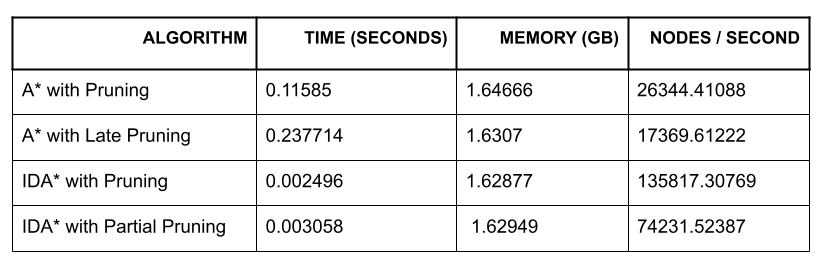
\includegraphics[scale=0.3]{hanois12D/tabla1.png} 
      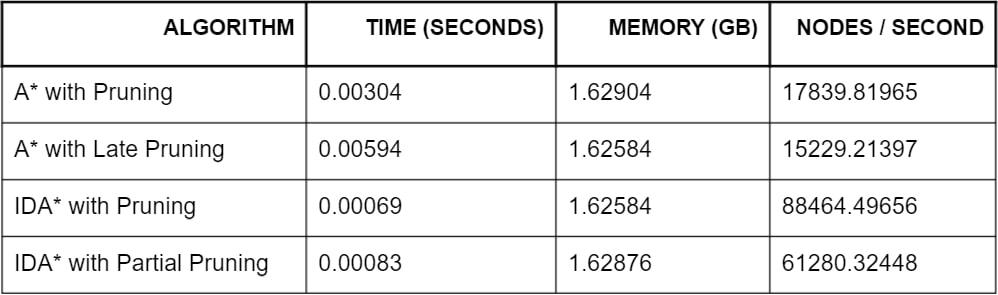
\includegraphics[scale=0.32]{hanois12D/12h_tabla_prom.jpg}\\
      \textit{\small{Tablas 6 y 7. A la izquierda, tiempo, memoria y n\'umero de nodos 
      expandidos en el caso de prueba dif\'icil de las Torres de Hanoi con 12 Discos para 
      cada algoritmo de b\'usqueda. A la derecha, promedio del tiempo, memoria y
      n\'umero de nodos expandidos entre los casos f\'aciles de las Torres de Hanoi
      con 12 Discos para cada algoritmo de b\'usqueda.}}\\
      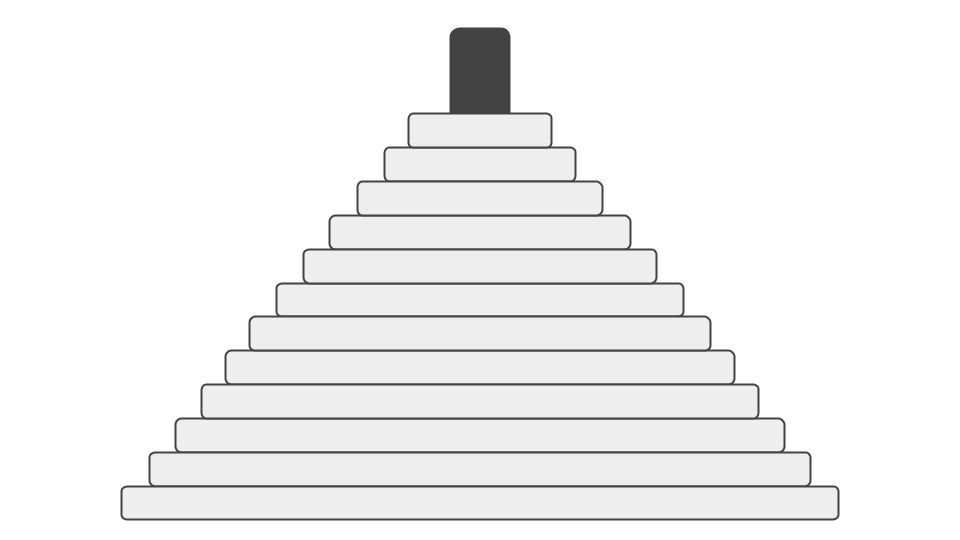
\includegraphics[scale=0.2]{hanois12D/pdb.png}
      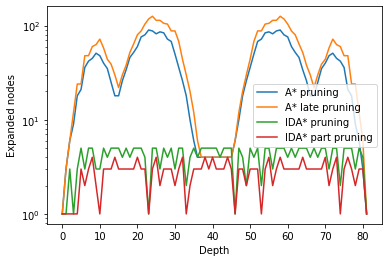
\includegraphics[scale=0.4]{hanois12D/hanois12D.png}
      \\
      \small{\textit{Figuras 6 y 7. A la izquierda, representaci\'on de los
      PDBs que usamos para las Torres de Hanoi con 12 Discos. B\'asicamente
      usamos un solo PDB que almacena todo el puzzle. A la derecha, N\'umero 
      de nodos expandidos por profundidad en el caso de prueba dif\'icil de
      las Torres de Hanoi con 12 Discos por cada algoritmo de b\'usqueda.}}
    \end{figure*}
    
  \subsection{Towers of Hanoi 4 Pegs - 14 Disks}
    Para las Torres de Hanoi con 14 Discos usamos como heur\'istica PDBs no aditivos, 
    particionando el puzzle tal como se muestra en \textit{Figura 8}. Para este puzzle
    decidimos usar un caso dif\'icil y otro medio dif\'icil, pues IDA* es muy poco
    eficiente en comparaci\'on a A* para resolver este problema, entonces en el dif\'icil 
    probamos \'unicamente A* para sacarle todo su potencial, y en el caso medio-dif\'icil 
    estudiamos tanto A* como IDA*.
    
    \begin{verbatim}
    4 4 4 4 4 4 4 4 4 2 2 2 2 2  (57)
    4 4 4 4 4 4 4 4 4 4 4 4 4 4  (113)
    \end{verbatim}
    
    Lo mas importante que se puede notar en la \textit{Tabla 8} es la diferencia en
    eficiencia entre A* e IDA* para este puzzle, tardando el primero menos de un 
    segundo para resolver el caso medio-dif\'icil, mientras que IDA* tard\'o cerca
    de una hora. La raz\'on de esto la podemos observar en la \textit{Figura 9}, 
    donde el n\'umero de estados expandidos por IDA* es del orden de $10^8$, mientas
    que A* apenas llega a $10^3$. Sin embargo, a partir de una profundidad de 20,
    el n\'umero de nodos expandidos por IDA* decrece abruptamente, y se mantiene en 
    el orden de los 10 nodos hasta llegar a la soluci\'on. Creemos que la raz\'on de 
    esto es que para el paso n\'umero 20 los dos bloques m\'as pesados ya se encuentran
    en la posici\'on correcta, por lo que el primer bloque de la heur\'istica, el 
    que se encuentra a la izquierda de la \textit{Figura 8}, pasa a convertirse en 
    el problema entero, llegando a una caso muy parecido al de las Torres de Hanoi
    con 12 discos. Lo que apoya nuestra teor\'ia es que desde la profundidad 20,
    la \textit{Figura 9} es muy parecida a la \textit{Figura 7}. \\
    
    Otra cosa por destacar es que la ineficiencia de IDA* en este puzzle coincide 
    con el hecho de que las Torres de Hanoi es el puzzle con crecimiento m\'as lento 
    y longitud de soluciones m\'as largo que hemos analizado.\\
    
    Por otro lado, A* con poda total fue m\'as eficiente que A* con poda tard\'ia,
    tal como se muestra en la \textit{Tabla 9}. Siendo por lo tanto, el m\'as
    eficiente en este algoritmo. Adem\'as, aunque no lo mostramos aqu\'i, para 
    los casos de prueba f\'aciles, todos los algoritmos de b\'usqueda tardan
    pr\'acticamente nada, pero el alg\'un cambio en alg\'uno de los dos bloques
    m\'as pesados hace que IDA* pase una gran cantidad de tiempo analizandolo. Es por eso 
    que decidimos que con estos 2 casos de prueba eran suficientes para realizar 
    nuestro an\'alisis.
    
    \begin{figure*}[t!]
      \centering
      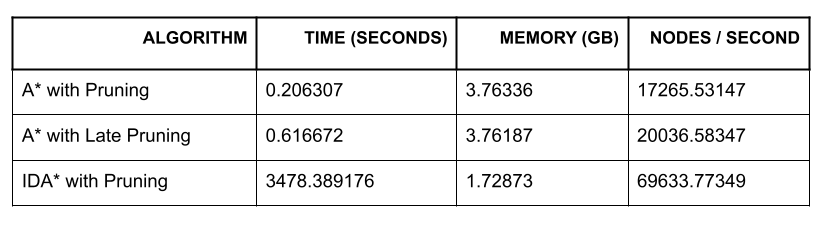
\includegraphics[scale=0.3]{hanois14D/tabla_medio.png}
      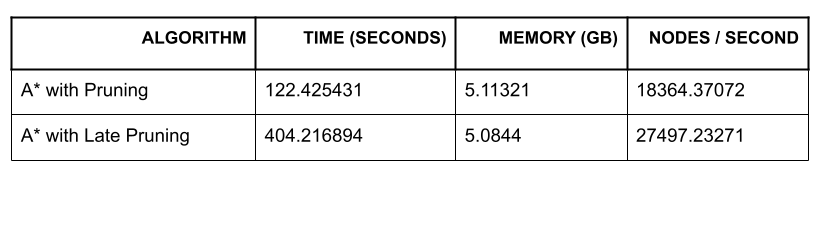
\includegraphics[scale=0.3]{hanois14D/tabla_dificil.png}\\
      \textit{\small{Tablas 8 y 9. A la izquierda y derecha tiempo, 
      memoria y n\'umero de nodos expandidos en el caso de prueba medio-dif\'icil y dif\'icil
      respectivamente de las Torres de Hanoi con 14 Discos.}}\\
      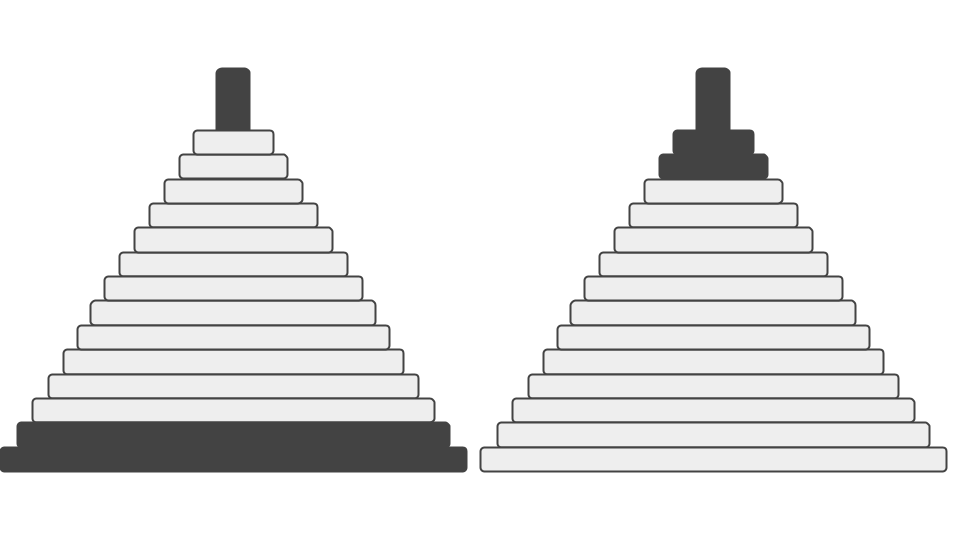
\includegraphics[scale=0.2]{hanois14D/pdb.png}
      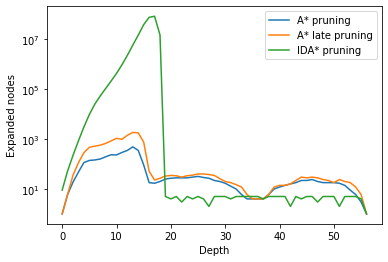
\includegraphics[scale=0.4]{hanois14D/hanois14_medium.png} 
      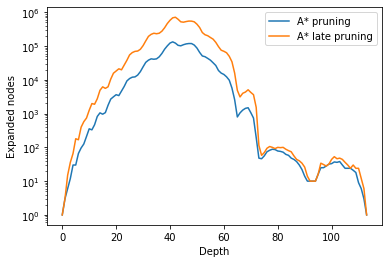
\includegraphics[scale=0.4]{hanois14D/hanois14_hard.png} \\
      \textit{\small{Figuras 8, 9 y 10. A la izquierda, representaci\'on de los PDBs
      usados para la heur\'istica de las Torres de Hanoi con 14 Discos. En el medio y a la derecha, n\'umero de nodos expandidos por profundidad en los casos de prueba
      medio-dif\'icil y dif\'icil respectivamente de las Torres de Hanoi con 14 Discos.}}
    \end{figure*}

  \subsection{Towers of Hanoi 4 Pegs - 18 Disks}
    Para las Torres de Hanoi con 18 Discos usamos como heur\'istica PDBs no aditivos, 
    particionando el puzzle tal como se muestra en \textit{Figura 11}. Para este puzzle
    el caso de prueba dif\'icil solo fue probado sobre A*, pues IDA* tard\'o casi una 
    hora en un caso de las Torres de Hanoi con 14 Discos cuando A* tard\'o menos de 
    un segundo. Por lo que para este puzzle podr\'ia tardar una cantidad exagerada de
    tiempo. Lo 5 casos de pruebas f\'aciles y el dif\'icil escogidos junto a la 
    longitud de sus soluciones fueron
    
    \begin{verbatim}
    3 1 1 1 1 1 1 1 1 1 1 1 1 1 1 1 1 1  (1)
    4 3 4 1 1 1 1 1 1 1 1 1 1 1 1 1 1 1  (4)
    2 4 3 2 1 1 1 1 1 1 1 1 1 1 1 1 1 1  (6)
    2 2 1 2 1 4 4 1 1 1 1 1 1 1 1 1 1 1  (18)    
    1 4 4 4 4 3 4 4 1 1 1 1 1 1 1 1 1 1  (29)
    1 2 2 1 2 4 4 2 3 2 4 1 4 1 1 1 1 1  (77)
    \end{verbatim}
    
    Para este puzzle ocurre pr\'aticamente lo mismo que con las Torres de Hanoi con
    14 discos, si los 6 discos m\'as pesados est\'an en la posici\'on correcta, entonces
    la primera heur\'istica guiar\'a al algoritmo directo a la soluci\'on sin hacerle
    expandir muchos nodos, tal como se ve en los tiempos de ejecuci\'on de la 
    \textit{Tabla 10}, los cuales son muy bajos. Sin embargo, mover un solo disco de
    los 6 m\'as pesados hace que la b\'usqueda se vuelva bastante extensa. En la 
    \textit{Tabla 11} se nota como A* pasa de tardar menos de 1 segundo a 34 segundos
    moviendo un solo bloque. Considerando el rendimiento de IDA* en las Torres de Hanoi 
    con 14 discos, no lo probamos con casos dif\'iciles para este puzzle pues el tiempo
    de busqueda se vuelve demasiado largo. \\
    
    Al igual que en el puzzle anterior, A* obtuvo el mejor rendimiento. Algo interesante
    de las gr\'asficas de A* en las Torres de Hanoi, es que todas presentan un 
    comportamiento ondulatorio, a diferencia de los N Puzzle que eran cuadr\'aticos
    invertidos. Esto puede deberse a que hay etapas en el puzzle en las que la heur\'istica
    logra guiar mejor a los algoritmo.
    
    \begin{figure*}[t!]
      \centering
      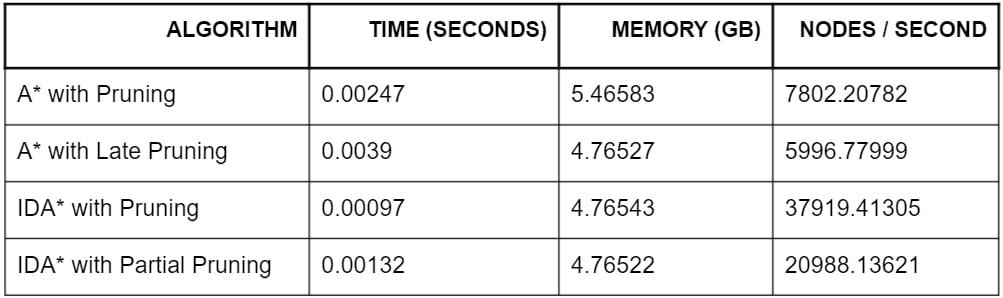
\includegraphics[scale=0.32]{hanois18D/18h_tabla_prom.jpg}
      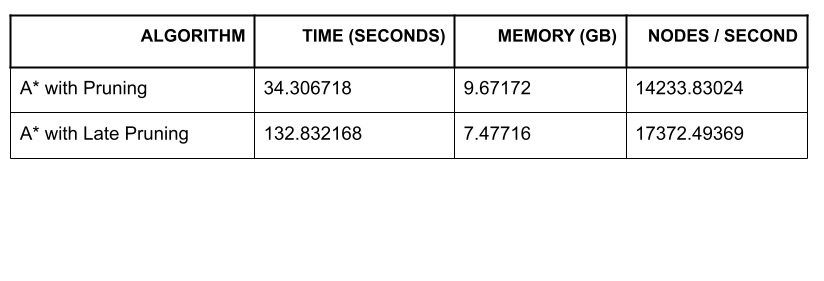
\includegraphics[scale=0.3]{hanois18D/tabla_hard.png}\\
      \textit{\small{Tablas 10 y 11. A la izquierda promedio de tiempo, memoria y 
      n\'umero de nodos expandidos en los 5 casos de pruebas f\'aciles de las Torres de Hanoi 
      con 18 Discos por cada algoritmo de b\'usqueda. A la derecha memoria y
      n\'umero de nodos expandidos en el caso de prueba dif\'icil de las Torres
      de Hanoi con 18 Discos.}}\\
      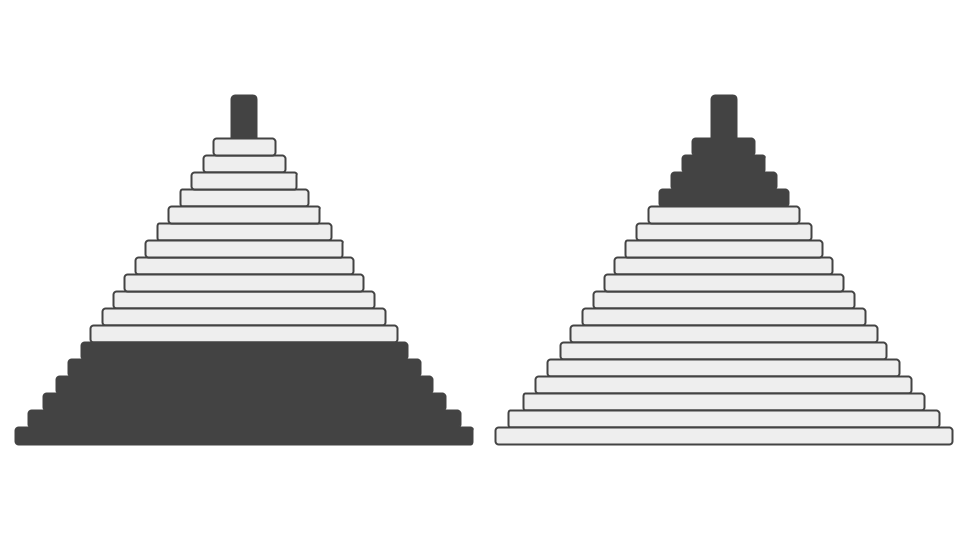
\includegraphics[scale=0.2]{hanois18D/pdb.png}
      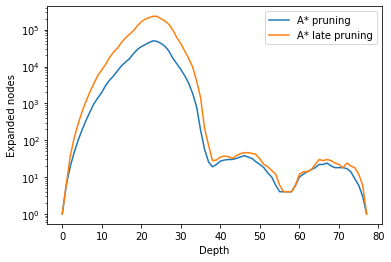
\includegraphics[scale=0.4]{hanois18D/hanois18_hard.png} \\
      \textit{\small{Figuras 11 y 12. A la izquierda, representaci\'on de los PDBs
      usados para la heur\'istica de las Torres de Hanoi con 18 Discos. A la derecha, n\'umero de nodos expandidos por profundidad en el caso de prueba
      dif\'icil de las Torres de Hanoi con 18 Discos usando A*.}}
    \end{figure*}
    
  \subsection{Top Spin 12 Tokens - Turntable of length 4}
    Para el Top Spin con 12 Tokens usamos como heur\'istica PDBs no aditivos, 
    particionando el puzzle tal como se muestra en \textit{Figura 13}. Los 5 casos de pruebas (todos dif\'iciles) escogidos junto a la 
    longitud de sus soluciones fueron
    
    \begin{verbatim}
    4 11 5 3 8 6 7 10 1 2 9 12  (9)
    11 1 6 5 2 10 9 8 4 7 3 12  (7)
    3 4 8 11 7 1 6 10 2 9 5 12  (8)
    2 6 7 5 11 1 10 9 8 3 4 12  (9)
    10 8 1 11 5 7 6 9 3 4 2 12  (10)
    \end{verbatim}
    
    No hay mucho que decir en este puzzle ya que, al poder almacenar todo
    el puzzle en un solo PDB, entramos en el mismo caso que las Torres de
    Hanoi con 12 Discos. La heur\'istica guiar\'a a los algoritmos 
    directamente a la soluci\'on sin mucha desviaci\'on, haciendo que el
    n\'umero de nodos expandidos en total sea bastante bajo independientemente
    de la dificulta del caso de prueba, por eso escogimos todos esos casos 
    con la mayor dificultad posible. Los resultados se muestran en las 
    \textit{Tablas 12 y 13}. Lo \'unico importante a mencionar es que, a
    diferencia de las Torres de Hanoi con 12 discos, en este caso el n\'umero
    de nodos expandidos por A* fue menor que IDA*.
    
    \begin{figure*}[t!]
      \centering
      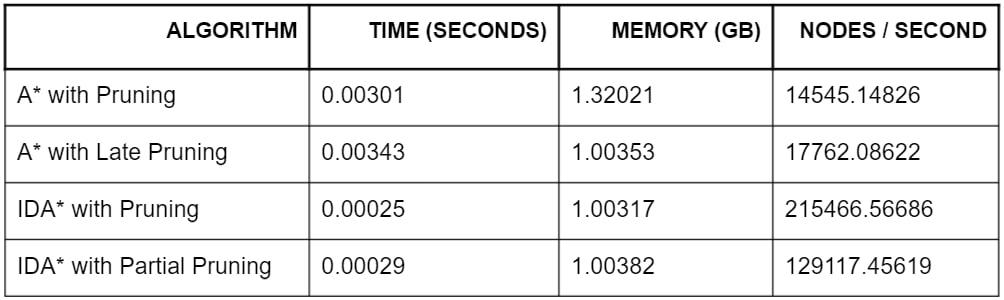
\includegraphics[scale=0.32]{topspin12T/12ts_tabla_prom.jpg}\\
      \textit{\small{Tablas 12. Promedio en tiempo, memoria y n\'umero de nodos expandidos por segundo entre los 5 caso de pruebas dif\'iciles de Top Spin con 12 Tokens para cada algoritmo de busqueda.}}\\
      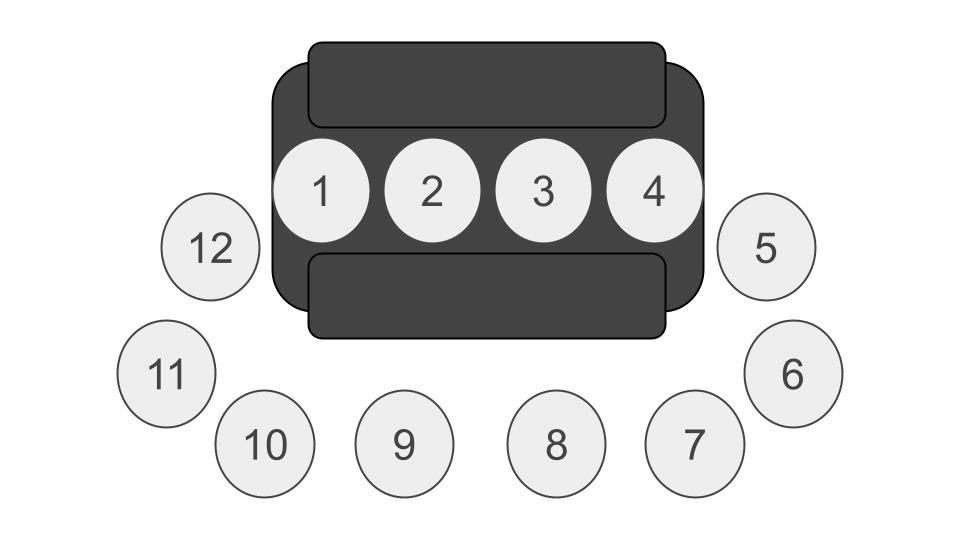
\includegraphics[scale=0.2]{topspin12T/pdb.png}
      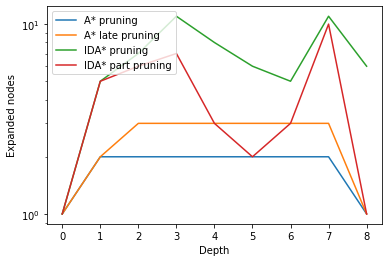
\includegraphics[scale=0.4]{topspin12T/topspin12.png} \\
      \small{\textit{Figuras 13 y 14. A la izquierda, representaci\'on de los
      PDBs que usamos para Top Spin con 12 Tokens. B\'asicamente
      usamos un solo PDB que almacena todo el puzzle. A la derecha, N\'umero 
      de nodos expandidos por profundidad en el caso de prueba dif\'icil de
      Top Spin con 12 Tokens por cada algoritmo de b\'usqueda.}}
    \end{figure*}

  \subsection{Top Spin 14 Tokens - Turntable of length 4}
    Para el Top Spin con 14 Tokens usamos como heur\'istica PDBs no aditivos, 
    particionando el puzzle tal como se muestra en \textit{Figura 13}. Los 5 casos de pruebas (todos dif\'iciles) escogidos junto a la 
    longitud de sus soluciones fueron
  
    \begin{verbatim}
    8 5 13 12 1 4 9 10 3 7 2 11 6 14 (11)
    4 7 13 3 9 2 8 6 10 1 5 12 11 14 (10)
    3 2 8 7 5 1 12 6 9 10 13 11 4 14 (11)
    11 12 4 3 6 10 9 8 13 7 1 5 2 14 (9)
    1 12 10 13 9 8 5 2 3 6 4 11 7 14 (11)
    \end{verbatim}
    
    A pesar de que no todo el puzzle cabe en un solo PDB, igualmente los
    casos de prueba se resuelven en pr\'acticamente nada de tiempo
    independientemente de su dificultas. Por eso decidimos usar 5
    casos de prueba dif\'iciles, cuyos resultados se muestran en la
    \textit{Tabla 13}. Incluso podemos notar en la \textit{Figura 15}
    que el n\'umero de nodos expandidos por profundidad es del orden
    de $10^3$, mucho menor en comparaci\'on a los otros puzzle. Debido
    a esto, no hay mucho que comparar entre los distintos algoritmos
    de b\'usquedas. Todos son tan eficientes que la diferencia entre 
    ellos es pr\'acticamente nula. 
    
    \begin{figure*}[t!]
      \centering
      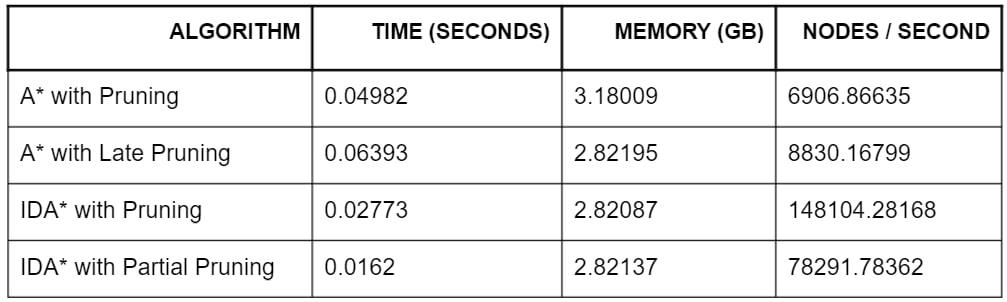
\includegraphics[scale=0.3]{topspin14T/14ts_tabla_prom.jpg} \\
      \textit{\small{Tabla 13. Promedio de tiempo, 
      memoria y n\'umero de nodos expandidos en los 5 casos de prueba
      f\'aciles de Top Spin con 14 Tokens por cada algoritmo de b\'usqueda.}}\\
      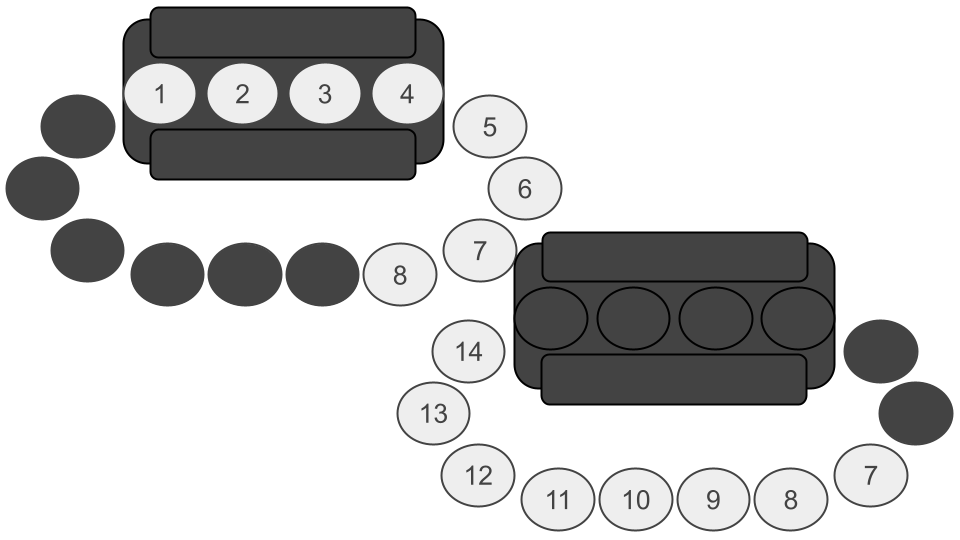
\includegraphics[scale=0.2]{topspin14T/pdb.png}
      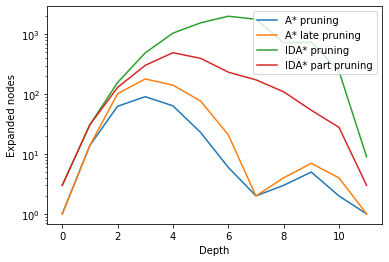
\includegraphics[scale=0.4]{topspin14T/topspin14.png} \\
      \small{\textit{Figuras 15 y 16. A la izquierda, representaci\'on de los
      PDBs que usamos para Top Spin con 14 Tokens. A la derecha, N\'umero 
      de nodos expandidos por profundidad en el caso de prueba dif\'icil de
      Top Spin con 14 Tokens por cada algoritmo de b\'usqueda.}}
    \end{figure*}
    
    \newpage

  \subsection{Top Spin 17 Tokens - Turntable of length 4}
    Para el Top Spin con 17 Tokens usamos como heur\'istica PDBs no aditivos, 
    particionando el puzzle tal como se muestra en \textit{Figura 13}. Los 5 casos de pruebas (todos dif\'iciles) escogidos junto a la 
    longitud de sus soluciones fueron
    
    \begin{verbatim}
      10 5 3 16 11 8 1 4 6 13 9 2 15 14 7 12 17 (15)
      16 3 14 7 2 5 9 1 12 8 15 10 13 6 11 4 17 (15)
      10 16 11 4 12 9 14 1 15 13 3 2 5 8 6 7 17 (15)
      9 12 13 1 15 8 3 11 5 14 7 16 4 2 6 10 17 (15)
      8 11 4 3 6 7 9 14 13 1 16 5 2 15 12 10 17 (15)
    \end{verbatim}
    
    Al igual que el puzzle anterior, solo escogimos casos de prueba
    dif\'iciles pues se resuelven con relativa facilidad, tal como
    se muestra en la \textit{Figura 14}. Sorprendentemente, el 
    algoritmo con mejor rendimiento y por mucho fue el de IDA* con
    poda parcial de duplicados, llegando a ser hasta 5 veces
    m\'as rapido que A* con poda total de duplicados, tal vez sea
    porque, entre todos los puzzles, este es el que tiene un 
    crecimiento mas elevado y una longitud de soluciones corta.
    Sin embargo, el que tuvo peor rendimiento fue IDA* con 
    eliminaci\'on total de duplicados, incluso podemos notar en 
    la \textit{Figura 18} que el n\'umero de nodos que expandi\'o
    es significativamente mayor que el del resto de los algoritmos.
    
    \begin{figure*}[t!]
      \centering
      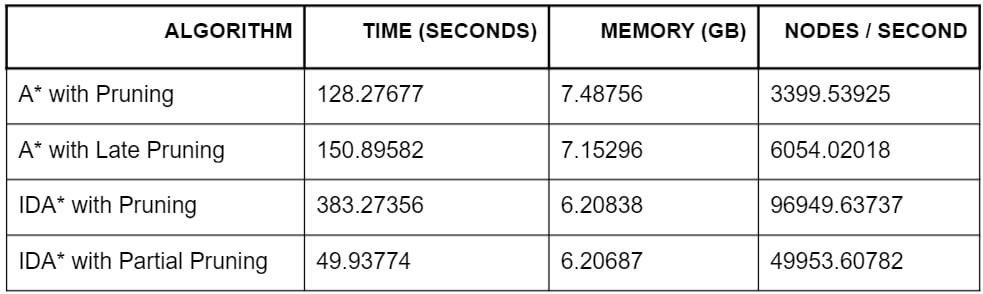
\includegraphics[scale=0.32]{topspin17T/17ts_tabla_prom.jpg}
      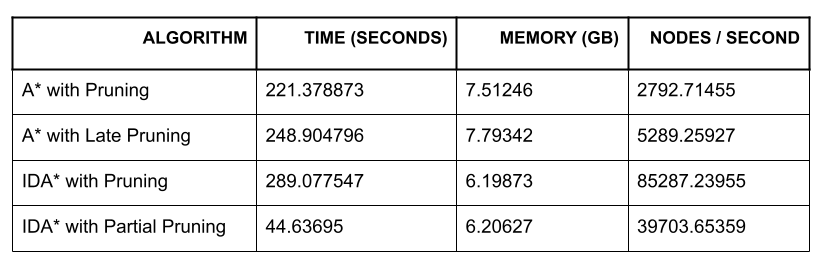
\includegraphics[scale=0.3]{topspin17T/tabla.png}\\
      \textit{\small{Tablas 14 y 15. A la izquierda, promedio de tiempo, 
      memoria y n\'umero de nodos expandidos en los 5 casos de prueba
      f\'aciles de Top Spin con 17 Tokens por cada algoritmo. A la 
      derecha, tiempo, memoria y n\'umero de nodos expandidos en el caso de 
      prueba dif\'icil de Top Spin con 17 Tokens para cada algoritmo de 
      b\'usqueda.}}\\
      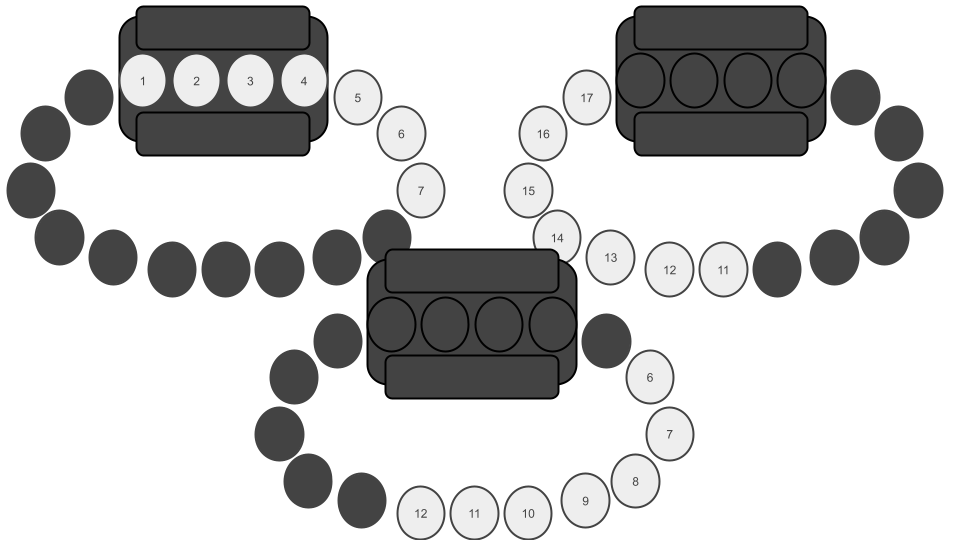
\includegraphics[scale=0.2]{topspin17T/pdb.png}
      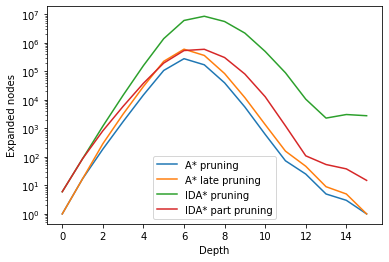
\includegraphics[scale=0.4]{topspin17T/topspin17.png} \\
      \small{\textit{Figuras 17 y 18. A la izquierda, representaci\'on de los
      PDBs que usamos para Top Spin con 17 Tokens. A la derecha, N\'umero 
      de nodos expandidos por profundidad en el caso de prueba dif\'icil de
      Top Spin con 17 Tokens por cada algoritmo de b\'usqueda.}}
    \end{figure*}

  \subsection{Rubik's Cube}
    Para el Cubo de Rubik usamos como heur\'istica PDBs no aditivos, 
    particionando el puzzle tal como se muestra en \textit{Figura 19}. Los 5 casos de pruebas f\'aciles escogidos junto a la 
    longitud de sus soluciones fueron
    
    \begin{verbatim}
        O B G G B O G O W W Y B R Y B R B Y W Y O G R B R R G O Y W G R O G Y W W G 
        R Y B R Y B W W O O (10)
        
        B W G G B B O O Y O W B B Y Y Y W O O R R W B W G R G B Y G W Y Y W R R G G 
        O Y R G O O W R R B (8)

        O O R W B W R O Y Y Y B Y G W G G Y B G R R W B G G R O W W G W B B G B O Y 
        O R O Y Y O B R W R (8)
        
        R W W R R W R R G G G B G Y G Y B B B O O Y O B B B Y G Y G Y G Y O B O O O
        O Y W W W W W R R R (8)
        
        Y R R B W W O G Y G G O O O G B O O O Y B G R W R B G Y B B W G G Y B R B O 
        W R Y W W R R W Y Y (9)
    \end{verbatim}
    
    Lamentablemente no pudimos realizar un estudio sobre alg\'un
    caso de prueba dif\'icil debido a problemas de conectividad.
    Podemos notar gracias a la \textit{Tabla 16} que para los 
    casos f\'aciles de este puzzle IDA* es m\'as eficiente que A*,
    tal como ha sido en la mayor\'ia de los casos de prueba f\'aciles
    estudiados en este proyecto. Algo muy importante a destacar es
    que la generaci\'on de nodos por segundo para este puzzle es
    muy baja en comparaci\'on al resto de puzzle. Esto puede deberse
    al tama\~no en la representaci\'on de los estados (48 caracteres)
    y a lo complicada que son las reglas de transici\'on del cubo
    de rubik, las cuales involucran cambiar el estado de varias
    posiciones al mismo tiempo, cuando en los otros puzzle en general
    s\'olo una peque\~na fracci\'on del estado es modificado entre
    cada movimiento.
  
    \begin{figure*}[t!]
      \centering
      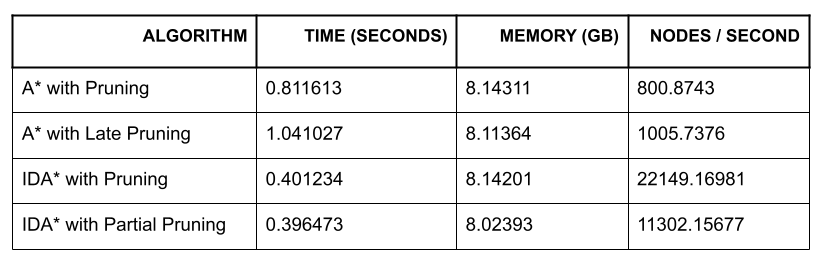
\includegraphics[scale=0.3]{rubik/tabla1.png} \\
      \textit{\small{Tabla 16. Promedio de tiempo, 
      memoria y n\'umero de nodos expandidos en los 5 casos de prueba
      f\'aciles del Cubo de Rubik por cada algoritmo de b\'usqueda.}}\\
      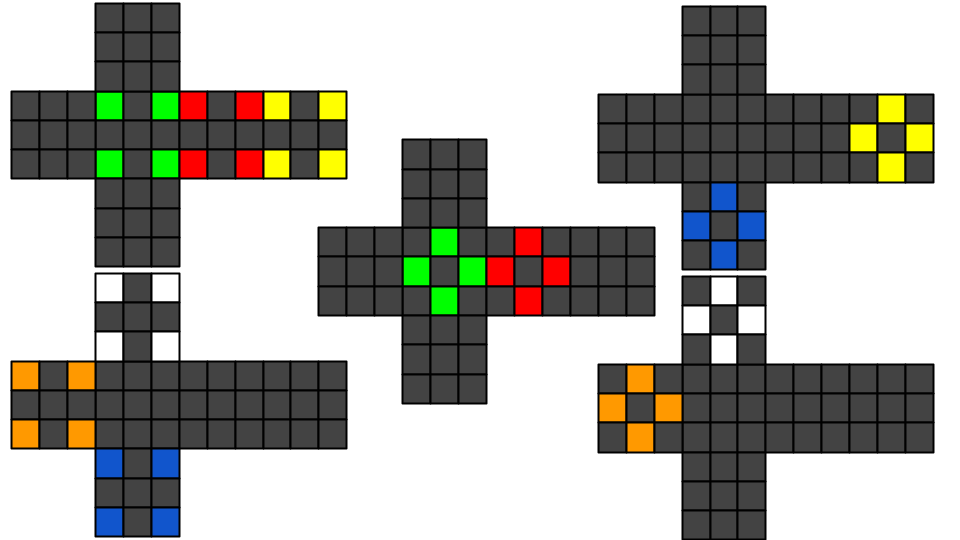
\includegraphics[scale=0.2]{rubik/pdb.png} \\
      \small{\textit{Figuras 19. Representaci\'on de los
      PDBs que usamos para el Cubo de Rubik}}
    \end{figure*}

\section{Detalles de Implementaci\'on}
  \subsection{NodesPriorityQueue}
    La clase \verb|NodesPriorityQueue| tiene 3 campos fundamentales:
    \begin{itemize}
      \item \verb|map<uint64_t, pair<unsigned, Node*>> hash| es un diccionario
      que mapea las valores de la tabla hash proporcionada por la API de PSVN
      a pares \verb|{V, N}| donde \verb|V| es el valor del nodo al que apunta
      \verb|N|.

      \item \verb|set<pair<unsigned, Node*>> ordered_nodes| es un conjunto de 
      pares \verb|{V, N}| con la misma definici\'on anterior. Cabe destacar 
      que el tipo de dato \verb|set| est\'a implementado en C++ como un arbol 
      rojo-negor, por lo que mantendr\'a ordenados los nodos seg\'un su valor 
      \verb|V|.

      \item \verb|unsigned (*f) (Node*)| es la funci\'on de evaluaci\'on de 
      los nodos.
    \end{itemize}

    As\'i, para buscar un nodo seg\'un su hash, simplemente tenemos que verificar
    que se encuentra en el campo \verb|hash|, lo cual es $O(1)$. Mientras que 
    para realizar el reemplazo, primero obtenemos el hash del estado que tiene 
    el nodo, luego, usando \verb|hash| obtenemos el par \verb|{V, N}|, y con ese 
    par, obtenemos el elemento que se encuentra en \verb|ordered_nodes|, y as\'i 
    realizamos el cambio en ambas estructuras en $O(\log n)$.

  
  \subsection{InformedSearchs}
    Para imprimir la memoria virtual usada actualmente se utiliza la estructura 
    \verb|struct sysinfo|, el cual, luego de aplicarle la funci\'on \verb|sysinfo|,
    almacena la memoria RAM y swap usada. As\'i, solo debemos imprimir la memoria 
    virtual inicial antes de correr el algoritmo y la memoria virtual justo antes 
    de terminar para saber aproximadamente cuanta memoria se us\'o. Para imprimir 
    el tiempo transcurrido se us\'o la funci\'on \verb|clock()|, marcando el tiempo 
    inicial e imprimiendo su diferencia con el tiempo final. \\

    Las funciones auxiliares \verb|apply_rule| y \verb|revert_rule| pueden parecer
    redundantes ya que la API de PSVN contiene las funciones \verb|apply_fwd_rule|
    y \verb|apply_bwd_rule| respectivamente. Sin embargo, estas dos \'ultimas tienen
    un problema cuando el estado al que se le aplicar\'a la regla y el estado que 
    almacenar\'a el sucesor son el mismo, probablemente porque es modificado mientras 
    es leido por la funci\'on. Es por esto que las funciones \verb|apply_rule| y 
    \verb|revert_rule| lo que hacen es generar un estado auxiliar copiando al estado 
    original, y lo usa como estado al que se le aplicar\'a la regla y almacena al 
    sucesor en el estado original. Estas son usadas por IDA* con eliminaci\'on parcial 
    de duplicados. \\

    La estructura \verb|NodesPriorityQueue| se us\'o en A* con eliminaci\'on de 
    duplicados, y realiza las funciones de almacenar los nodos ordenados seg\'un su 
    valor (costo del camino parcial m\'as la heur\'istica), y permite verificar la 
    existencia de un estado y la sustituci\'on de nodos con el mismo estado de forma 
    eficiente. \\

    Mientras que para A* con eliminaci\'on tard\'ia de duplicados se us\'o una tabla
    de hash que mapea los valores de hash para los estados dado por la API de PSVN 
    a costos parciales. As\'i, podemos verificar la existencia de un estado y su costo 
    almacenado de forma eficiente. \\ 

    Para IDA* con eliminaci\'on de duplicados se utiliz\'o una variable de tipo 
    \verb|set| que almacenaba los nodos que se encontraban en el camino actual. As\'i,
    solo basta con verificar si un nodo sucesor pertenece a dicho camino para saber 
    si se debe agregar o no.

  \subsection{PDBs}
    El proceso de generaci\'on de un PDB para un puzzle sigue los siguientes pasos:
    \begin{enumerate}
      \item Compilar el archivo \verb|abstractor.cpp| y \verb|psvn.cpp| de la API de 
      PSVN para obtener un archivo binario \verb|abstractor.out| que nos permita crear 
      la abstracci\'on que necesitamos.
      \item Utilizar \verb|abstractor.out| para generar un la abstracci\'on \verb|.psvn| 
      a partir del archivo \verb|.psvn| original y el archivo \verb|abstraction|.
      \item Ejecutar \verb|psvn2c| sobre el archivo \verb|.psvn| abstraido para generar 
      un archivo \verb|.c| que contiene las reglas del puzzle abstraido codificadas.
      \item Compilar el archivo \verb|dist.cpp| proporcionado por la API de PSVN junto 
      al \verb|.c| del paso anterior para generar un ejecutable \verb|.dist|.
      \item Ejecutar el archivo \verb|.dist|, el cual generar\'a un PDB codificado en 
      un archivo tal que cada l\'inea sigue el formato \verb|<VALUE> <STATE>|, donde 
      \verb|<VALUE>| es el costo m\'inimo desde el estado \verb|<STATE>| hacia el estado 
      objetivo. Este output es almacenado en un archivo \verb|.pdb| que puede llegar a 
      ser muy pesado.
      \item Eliminar el archivo \verb|.c| y \verb|.psvn| abstraido y luego copiar y 
      pegar el \verb|.psvn| original en el directorio actual. La raz\'on de hacer esto 
      es que para compilar el siguiente archivo necesitamos usar el psvn con las reglas 
      y estados originales.
      \item Compilar el archivo \verb|make_state_map| creado por nosotros el cual 
      inicializa una variable del tipo \verb|state_map_t| proporcionado por la API, y 
      por cada l\'inea del archivo \verb|.pdb| almacena en dicha variable el estado y 
      su valor. Luego de recorrer todo el archivo, almacena la variable de 
      \verb|state_map_t| en un archivo \verb|.state_map|.
      \item Ejecutamos \verb|make clean| para quedarnos \'unicamente con el archivo 
      \verb|.state_map|.
    \end{enumerate}

  \subsection{heuristics}
    Para evitar crear una funci\'on heur\'istica por cada puzzle del mismo tipo pero 
    con diferentes dimensiones, por ejemplo 3 funciones para Top Spin con 12, 14 y 17 
    tokens respectivamente, donde cada funci\'on ser\'a casi exactamente igual pero 
    cambiando el valor de algunas variables, decidimos utilizar variables globales 
    que definan el comportamiento de las heur\'isticas:

    \begin{itemize}
      \item \verb|vector<state_map_t*> pdbs| almacena los PDBs que se usar\'an en las 
      heur\'isticas. La funci\'on \verb|init_pdbs| permite cargar todos en \verb|pdbs|
      los archivos \verb|.state_map| que se encuentren en un directorio dado como 
      argumento. Los \verb|.state_map| son cargados en orden alfab\'etico. 

      \item \verb|unsigned (*f) (unsigned, unsigned)| es una funci\'on que indica la 
      relaci\'on entre heur\'isticas de bloques PDB, puede tomar el valor de 
      \verb|max_h| para agarrar el m\'aximo en caso de heur\'isitcas no aditivas, o 
      \verb|sum_h| para sumarlas en caso de heur\'isitcas aditivas. Las funciones que 
      realizan la asignaci\'on de \verb|f| son \verb|set_max| y \verb|set_sum|.

      \item Cada puzzle tiene su propia variable global \verb|partition| (pudiendo 
      ser de distinto tipo entre cada puzzle) que almacena la forma en que se 
      particionar\'a el puzzle para los PDBs. Es importante que el orden en el que 
      se encuentran los bloques de la partici\'on corresponda al orden en el que son 
      cargados los PDBs en la variable \verb|pdbs|, en caso contrario se obtendr\'a
      un bello y hermoso \verb|segmentation fault|. Por cada variante de un puzzle 
      existe una partici\'on correspondiente y una funci\'on que realiza la 
      asignaci\'on de la variable \verb|partition| global del puzzle gen\'erico a 
      la variable \verb|partition| del puzzle con dimensiones espec\'ificas. Por 
      ejemplo, para los NPuzzles existe una variable \verb|string **partition_Npuzzle|
      y para el 15Puzzle y 24Puzzle est\'an las variables 
      \verb|string partition_15puzzle[4][4]| y \verb|string partition_24puzzle[5][5]|
      junto a las funciones \verb|set_15puzzle| y \verb|set_24puzzle| respectivamente 
      que asignan a \verb|partition_Npuzzle| la partici\'on que corresponda.
    \end{itemize}

    Adem\'as, cada puzzle tiene su propia funci\'on \verb|make_state_abs| que toma un 
    estado y un bloque de la partici\'on y genera un nuevo estado abstraido seg\'un 
    dicho bloque. Una vez con estos elementos, las heur\'isticas de cada puzzle siguen 
    el mismo comportamiento: Reciben un esto, recorren el vector \verb|pdbs| y por cada 
    uno generamos un estado abstraido dado el bloque de la partici\'on correspondiente, 
    obtenemos el valor de dicho estado seg\'un el \verb|state_map| y actualizamos el 
    valor de la heur\'isitca seg\'un \verb|f|. 
    
\newpage
\section{Conclusi\'on}
    El rendimiento de A* e IDA* depende mucho del tipo de puzzle que
    querramos resolver y de la dificultad del caso de prueba. Tal
    como vimos con las Torres de Hanoi, complicar un poco un estado
    inicial puede llevar a que un algoritmo pase de correr en 
    segundos a tardar cerca de una hora. Sin embargo, podemos hacer
    algunas generalizaciones para saber cuando hay que usar A* o IDA*. La primera es verificar la longitud de las soluciones
    promedios de un puzzle, mientras mas largo sea, peor ser\'a el
    rendimiento de IDA*, pues este deber\'a recorrer todo el espacio
    de b\'usqueda hasta cada profundidad. Siguiendo la misma 
    l\'ogica, al ser m\'as dif\'icil un caso de prueba, generalmente
    significa que se necesitan m\'as pasos para resolverse, lo
    que termina perjudicando a IDA*. Ahora, si las longitudes de las
    soluciones es corta, IDA* es la mejor opci\'on, tal como vimos
    en el an\'alisis de Top Spin. \\
    
    Respecto a los PDBS, vimos lo \'utiles que pueden llegar a ser,
    sobre todo cuando es posible almacenar gran parte del puzzle
    en un solo PDB. Adem\'as, es importante saber como separar 
    en bloques al puzzle, pues una buena elecci\'on resultar\'a
    en una aceleraci\'on en la resoluci\'on de los problemas, as\'i
    como en las Torres de Hanoi la heur\'istica logr\'o orientar
    a IDA* directamente a la soluci\'on una vez los bloques m\'as 
    pesados estuvieron en la posici\'on correcta. Esto no hubiera
    sido posible si, por ejemplo, en lugar de escoger un bloque 
    de PDB que no incluyera los discos mas pesados, no se 
    incluyeran algunos discos livianos, entonces la heur\'istica
    no podr\'ia guiar al algoritmo directamente a la soluci\'on
    hasta que dichos discos estuvieran ordenados, pero al alcanzar
    ese punto o el puzzle ya esta casi resuelto, o se tendr\'an
    que desordenar para darle paso a los discos pesados. \\
    
    Hace falta hacer m\'as pruebas pues, debido a problemas de 
    conectividad, no logramos hacer todos los casos de prueba
    que queriamos analizar. Principalmente para los casos de prueba
    dif\'iciles, los cuales solo pudimos analizar uno por puzzle 
    (o ninguno en caso del Cubo de Rubik), por lo que pudimos
    haber estado estudiando un caso de prueba anormal, el cual 
    dar\'ia datos anormales no aptos para la generalizaci\'on. \\
    
    
\end{document}